\scanpage{24}
(donc pour tt partie quasi-compacte $K$ de $U$, $\exists i=i(K)\in\mathbb N$ tel que $X_i\cap K=\varnothing$). Alors $F=\Gamma(X,\underline F)$ satisfait à a) b) c) d) \deleted{\unsure{e)}} et aussi à e) si $X$ quasi-compact. Plus \unsure{gén.}, si $A\in\unsure{F}$, alors $F_A$ \inserted{$=$ ens des parties de $A$ qui sont loc. \unsure{induites} par des sections de $\underline F$} satisfait à a) b) c) d) \deleted{\unsure{e)}} (il satisfait à e) si ???).

\unsure{Ici} il est plus commode de postuler l'axiome suivant plus fort que e)

$(e_n)$ $\exists$ un entier $n$ tel que si \inserted{$U,$} $X_0\supset X_1\supset\cdots\supset X_n\supset X_{n+1}$ est comme dans $\unsure{e)_{\underline F}|e)}$ ci-dessus, alors on a $X_{n+1}=\varnothing$. (On dit que $X$ est de $\underline F$-dim $\leq n$)
\figure{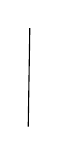
\begin{tikzpicture}\draw (0,0)--(.02,1.25);\end{tikzpicture}}
Alors tous les $F_A$ ($A$ \deleted{\unsure{loc$^t$}} fermé dans $X$) satisfont \deleted{\unsure{à}} $e_n)$, donc e).

\uline{NB} $\underline F$ est à priori $\supset$ le faisceau \uline{engendré} par $F=\Gamma(X,\underline F)$ et l'inclusion peut être stricte. \uline{Ex}: germes de parties analytiques d'un tore analytique de dim 2 sans fonctions méromorphes non constantes ---

Nous \deleted{\unsure{supposons}} \inserted{envisageons} maintenant une condition

f)
\mspage{25}
